\documentclass{article}
\usepackage[utf8]{inputenc}
\usepackage[T2A]{fontenc}
\usepackage[russian,english]{babel}
\usepackage{import}
\usepackage{scn}
\usepackage{graphicx} % Required for inserting images
\usepackage{float}
\usepackage{multicol}
\usepackage{subfig}
\usepackage{fancyhdr}
\usepackage{setspace}
\usepackage[numbers]{natbib}
\usepackage[top=20mm,columnsep=15pt]{geometry}%hmarginratio=1:1
\usepackage{titlesec}
\usepackage{titling}
\fancyhf{} % очищает все верхние и нижние колонтитулы.
\cfoot{\textbf{\thepage}}
\pagestyle{fancy}
\renewcommand{\footrulewidth}{0pt} 
\renewcommand{\headrulewidth}{0pt}
\title{\centering \vspace{-15mm} \huge \textbf{Interoperability as a Critical Component of the
Educational Process in Secondary Schools}}
\author{Alena Kazlova and Alexander Halavaty\\ \small
\textit{Belarusian State University}\\ \small
Minsk, Belarus\\ \small
Email: kozlova@bsu.by}
\date{}
\titleformat{\section}[block]{\normalsize \centering}{\thesection.}{0.4em}{}
\renewcommand\thesection{\Roman{section}}
\geometry{
  a4paper,
  left=25mm,
  right=22mm,
  top=20mm,
  bottom=20mm,%20mm
  hratio=1:1,
  vratio=1:1
}
\graphicspath{ {images/} }
\captionsetup{belowskip=2.5mm}
%\bibliography{images/biblio}

\setcounter{figure}{6}
\setcounter{page}{120}
%\title{Lab1}
%\author{dima.burbas}
%\date{September 2024}

\begin{document}
\begin{multicols}{2}
\begin{figure}[H]
    \centering
    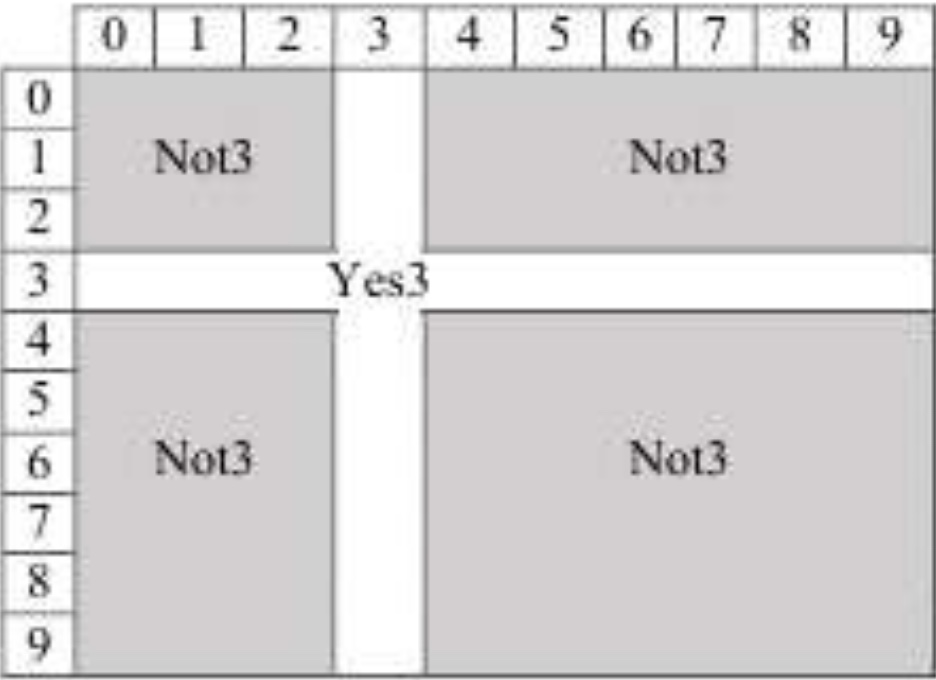
\includegraphics[width=0.7\linewidth]{images/Figure7.jpeg}
    \caption{\small Definition areas of Not3 and Yes3 classes.}
    \label{fig:enter-label}
\end{figure}
\fontsize{10pt}{12pt}\selectfont
\hspace{-1.5em}for automatic detection of hidden interpretable patterns
in the training data set. The revealed patterns can be used
then to construct a classification algorithm.
\par The learning algorithm for identifying combinations
of features that have the property of class distinction
is described. As a result of analyzing the training data
set, the informativeness estimates of combinations of
distinguishing features (from the point of view of classes)
are automatically calculated and a classifier is built.
\par Based on model data, the results of applying the
developed method to solve the classification problem are
presented.
\par
\renewcommand{\refname}{\centering References}
\fontsize{8pt}{9pt}\selectfont
\begin{thebibliography}{26}
\vspace{2.5mm}
\setlength{\itemsep}{0pt}
\bibitem{item1} D. Gurvits, A. N’yudzhent, F. Khalper Prosto o bol’shikh dannykh
[Big Data For Dummies], Moskow, Eksmo. 2015. 400 p.
\bibitem{item2} A. Vaigend, Big Data. Vsya tekhnologiya v odnoi knige [Big Data.
All the technology in one book], Moskow, Eksmo. 2018. 384 p.
\bibitem{item3} N. Marts, Dzh. Uorren Bol’shie dannye: printsipy i praktika postroeniya masshtabiruemykh sistem obrabotki dannykh v
real’nom vremeni [Big Data: Principles and best practices of
scalable realtime data systems], Moskow, OOO “I.D. Vil’yams”,
2016. 368 p.
\bibitem{item4} D. Silen, A. Meisman, M. Ali Osnovy Data Science i Big
Data. Python i nauka o dannykh [Introducing Data Science: Big
Data, Machine Learning, and more, using Python tools], Saint
Petersburg, Piter. 2017. 336 p.
\bibitem{item5} A.A. Barsegyan, M.S. Kupriyanov, I.I. Kholod Analiz dannykh i
protsessov [Data and Process Analysis], Saint Petersburg, BKhVPeterburg. 2009. 512 p.
\bibitem{item6} A.G. D’yakonov Analiz dannykh, obuchenie po pretsedentam,
logicheskie igry, sistemy WEKA, RapidMiner i MatLab [Data
analysis, learning by precedents, logic games, WEKA, RapidMiner and MatLab systems], Moskow, Izdatel’skii otdel fakul’teta
VMK MGU imeni M.V. Lomonosova. 2010. 278 p.
\bibitem{item7} Dzh. Gras Data Science. Nauka o dannykh s nulya [Data Science
from Scratch], Saint Petersburg, BKhV-Peterburg. 2017. 416 p.
\bibitem{item8} K. Fukunaga Vvedenie v statisticheskuyu teoriyu raspoznavaniya
obrazov [Introduction to Statistical Pattern Recognition], Moskow,
Nauka, 1979. 368 p.
\bibitem{item9} K.M. Bishop Raspoznavanie obrazov i mashinnoe obuchenie [Pattern Recognition and Machine Learning], Moskow, Dialektika,
2020. 960 p.
\bibitem{item10} V.V. Myasnikov Raspoznavanie obrazov i mashinnoe obuchenie.
Osnovnye podkhody [Pattern recognition and machine learning.
Basic approaches], Samara, Izdatel’stvo Samarskogo universiteta,
2023. 196 p.
\bibitem{item11} A.D. Zakrevskii Logika raspoznavaniya [Recognition logic],
Minsk, Nauka i tekhnika, 1988. 118 p.
\bibitem{item12} N.G. Zagoruiko Prikladnye metody analiza dannykh i znanii
[Applied methods of data and knowledge analysis], Novosibirsk,
IM SO RAN, 1999. 270 p.
\bibitem{item13} A.V. Bobkov Sistemy raspoznavaniya obrazov [Pattern recognition systems], Moskow, MGTU imeni N.E. Baumana, 2018. 187p.
\bibitem{item14} V. Krasnoproshin, A. Karkanitsa, V. Rodchenko Pattern Recognition Based on Classes Distinctive Features. Proc. of 15-th
International Conference “Pattern Recognition and Information
Processing”, 2021, pp. 22-25.
\bibitem{item15} V.I. Vasil’ev Problema obucheniya raspoznavaniyu obrazov :
Printsipy, algoritmy, realizatsiya [The problem of teaching pattern recognition: Principles, algorithms, implementation], Kiev,
Vyshcha shkola, 1989. 64 p.
\bibitem{item16} V. Krasnoproshin, V. Rodchenko Obuchenie po pretsedentam na
osnove analiza svojstv priznakov [Learning by precedents based
on the analysis of the features]. Doklady BGUIR, 2017, no 6, pp.
35-41.
\bibitem{item17} Dzh. Tu, R. Gonsales Printsipy raspoznavaniya obrazov [Principles of pattern recognition], Moskow, Mir, 1978. 411 p.
\bibitem{item18} S. Rashka Python i mashinnoe obuchenie [Python and machine
learning], Moskow, DMK Press, 2017. 418 p.
\bibitem{item19} V.V. Krasnoproshin, V.G. Rodchenko Klassifikatsiya na osnove
prostranstv reshenii [Classification based on decision spaces].
Doklady BGUIR, 2019, no 6, pp. 20-25.
\bibitem{item20} Yu.I. Zhuravlev Ob algebraicheskom podkhode k resheniyu
zadach raspoznavaniya ili klassifikatsii [On an algebraic approach
to solving recognition or classification problems]. Problemy kibernetiki [Problems of cybernetics], 1978, no 33, pp. 5-68.
\bibitem{item21} P. Flakh Mashinnoe obuchenie. Nauka i iskusstvo postroeniya
algoritmov, kotorye izvlekayut znaniya iz dannykh [Machine
learning. The science and art of building algorithms that extract
knowledge from data], Moskow, DMK Press, 2015. 400 p.
\bibitem{item22} V. Krasnoproshin, A. Karkanitsa, V. Rodchenko Implementation
of the KD-Agent for Knowledge Ecosystem. Otkrytye semanticheskie tekhnologii proektirovaniya intellektual’nykh system [Open
semantic technologies for intelligent systems], 2021, pp. 59-62.
\bibitem{item23} L.A. Belozerskii Sovremennyi vzglyad na gipotezu kompaktnosti
[Modern view of the compactness hypothesis]. Iskusstvennyi
intellekt [Artificial intelligence], 2005, no 3, pp. 6-12.
\bibitem{item24} V. Rodchenko Pattern Recognition: Supervised Learning on the
Bases of Cluster Structures. Proc. XIII International Conference
“Pattern Recognition and Information Processing”, 2016, pp. 106-
113.
\bibitem{item25} V. Rodchenko Automatic Detection of Hidden Regularities Based
on the Study of Class Properties. Pattern Recognition and Image
Analysis, 2020, vol. 30, no 2, pp. 224-229.
\bibitem{item26} V.V. Krasnoproshin, V.G. Rodchenko Klasternye struktury i ikh
primenenie v intellektual’nom analize dannykh [Cluster structures
and their application in data mining]. Informatika [Informatics],
2016, no 2, pp. 71-77.
\end{thebibliography}
\selectlanguage{russian}
\titlespacing*{\section}{5pt}{5pt}{0pt}{}
\section*{\centering\fontsize{8pt}{9pt}\selectfont\textbf{ПРИНЦИП ОБЩНОСТИ СВОЙСТВ И
KD-КЛАССИФИКАЦИЯ}}
\begin{center}
\fontsize{9pt}{9pt}\selectfont
{Краснопрошин В.В., Родченко В. Г., Карканица А. В.}
\end{center}
\vspace{-0.5em}
\fontsize{9pt}{9pt}\selectfont
\parВ работе исследуется актуальная проблема автоматического обнаружения скрытых интерпретируемых закономерностей в интеллектуальных системах. Концептуальную
основу процесса обучения по прецедентам определяют способы описания и разделения классов. Известны три базовых
принципа: перечисления членов класса, общности свойств
и кластеризации. Предлагается оригинальный метод реализации принципа общности свойств, основанный на поиске
сочетаний признаков, обеспечивающих различение классов.
Эффективность подхода подтверждается результатами численного эксперимента.
\vspace{-4mm}
\begin{flushright}
Received 14.03.2024
\end{flushright}
\end{multicols}
\newpage
\maketitle
\begin{multicols}{2}
\fontsize{8pt}{9pt}\selectfont
\textbf{\textit{Abstract}—The paper presents some results of an analysis
of the role of the development of interoperability, cognitive abilities and emotional intelligence in children in a
modern school. The importance and ways of introducing
technological tools with capabilities for interaction and data
exchange to optimize the educational process are discussed.
The significance of the development of cognitive abilities
and emotional intelligence of students and the impact of
this on their academic achievements and social adaptation
are also considered.}
\par \textbf{\textit{Keywords}—Education, interoperability, cognitive abilities,
emotional intelligence, intelligent educational systems} \par
\fontsize{10pt}{12pt}\selectfont
\vspace{-1.5em}
\section{Introduction}
\vspace{-0.5em}
\hspace{1em}School education is an initial and very important stage,
which forms the basis for all further development of an individual’s education, exerting a significant influence not
only on his future activities as a specialist in a particular
sector of the economy, but also as an individual, a member of society. It is at school that “the intellect is formed,
which is a combination of various functions (sensoryperceptual, mnemological and attentive)” [1], and the
personality itself is formed. It is the complex development of the individual, the combination of professional,
technical, and personal, universal knowledge and skills
that determine the success of a modern person, his ability
not only for his own development and improvement, but
also for the development and improvement of society in
all forms of its existence [2].
\par In the process of digitalization of education, a variety
of tools, methods and technologies are used, largely
based on the use of artificial intelligence algorithms.
Such types of training as network and electronic are
being developed, which include not only the direct educational part, but also means of automating the learning
process itself. At the same time, often “behind the scenes”
there remains such an important issue as the education of
an individual capable of thinking creatively, being able
to organize one’s own learning process, and also working
in a team, distributing tasks, negotiating, explaining his
point of view, justifying his decisions. In fact, when
considering the development of digital platforms and
intelligent educational systems, we should talk about the
human interoperability. It is becoming increasingly clear
that interoperability is necessary both to create a single
barrier-free information space based
on the principles
of openness, transparency, multi-purpose use of data,
technological neutrality, and to ensure the priority of user
interests, information security and protection of privacy
[3]. The study of the development of the properties of
interoperability, cognitive abilities and emotional intelligence starting from childhood is increasingly relevant
with the development of society and the transition to the
sixth technological order, in which the leading role is
given, along with information and nanotechnologies, to
cognitive sciences and socio-humanitarian technologies.
\par The main goal of the present paper is to give an analytical overview of the role and methods of development of
secondary school students’ cognitive abilities along with
the emotional intelligence and interoperability. Another
idea was to determine some basic concepts within the
interoperability as a subject area and the property of a
school student.
\section{\hspace{-0.5em} The cognitive abilities level and the interoperable
behaviour. State of art}
\hspace{1em}According to the American Psychological Association
Dictionary of Phychology, cognitive ability is defined as
the skills involved in performing the tasks associated with
perception, learning, memory, understanding, awareness,
reasoning, judgment, intuition, and language [4].
\par People are engaged at every step in the data value
chain in collecting, analyzing, interpreting, and using
data. In many cases, people themselves are data points.
All these people bring perspectives, values, world views,
and expectations, which are also embedded in political
and organizational cultures. If we want data to work
together, we need people to work together. We need
human interoperability [5], [6].
\par Emotional Intelligence (EI) is the ability to manage
both your own emotions and understand the emotions of
people around you. There are five key elements to EI:
self-awareness, self-regulation, motivation, empathy, and
social skills. People with high EI can identify how they
are feeling, what those feelings mean, and how those
emotions impact their behavior and in turn, other people.
It’s a little harder to “manage” the emotions of other
people — you can’t control how someone else feels or
\newpage
behaves. But if you can identify the emotions behind their
behavior, you’ll have a better understanding of where
they are coming from and how to best interact with
them [7].
\par Let us consider some characteristics of preschoolers
and schoolchildren, depending on their age, from the
point of view of developing the ability for interoperable
behavior.
\par Even in preschool age — about 4-5 years — the
child begins to understand that other people may have
opinions, thoughts, and desires that are different from his
own. This ability to understand and accept differences
in people’s thinking develops as we grow older. Some
researchers note that the better developed such mental
empathy is, the higher a person’s academic performance
at school and university [1], [2], [4], [5], [6], [7], [8],
[9], [10]. This ability helps build relationships of mutual
understanding and involvement, participation between
mentors and classmates, leading to the perception and
understanding of tasks and requirements.
\par The younger schoolchild (6 – 10 years old) is characterized primarily by readiness for educational activities,
i. e. he is ready to study systematically. It is also the
ability to accept new responsibilities, which underlies
the educational motivation of a primary school student.
This period is the most important for the development
of aesthetic perception, creativity and the formation of a
moral and aesthetic attitude towards life, which is fixed
in a more or less unchanged form for the rest of life. In
elementary school, the younger student develops forms
of thinking that ensure the further assimilation of various
knowledge and the development of thinking. At this age,
you can also develop the student’s self-organization and
self-discipline skills, for example, through group games,
encouraging healthy curiosity, and interest in all kinds of
creative activities.
\par In middle school age (from 10–11 to 14–15 years),
communication with peers plays a decisive role. The
leading types of activities are educational, social and
organizational, sports, creative, and labor [1]. During this
period, the child acquires significant social experience
and begins to comprehend himself as an individual in the
system of labor, moral, and aesthetic social relations. He
has a deliberate desire to take part in socially significant
work, become socially useful, and interact in a team.
\par In the period of early adolescence (from 14–15 to
17 years), value-orientation activity, which is determined
by the desire for independence, acquires key importance.
The main components of this period are friendship and
trusting relationships. This is the stage that many authors
call the final stage of personality maturation [1], [2],
when professional interests are clearly formed, theoretical
thinking, the ability for self-education, the ability to
reflect are developed, the level of aspirations is formed.
At this stage, a person is able to formulate his demands,
interact with other members of the team, forming personal connections, for example, friendship, sympathy.
\par Each of the stages of learning and growing up should
be accompanied by the acquisition of interaction skills
in teams, not so much for the purpose of competitively
achieving the result of joint activity, but for the purpose
of teaching a person to look for the best, including
joint, solutions to assigned tasks. That is, the main
goal and task of an interoperable person is the search
and implementation of the best solution in the given
conditions and given the available opportunities, and not
a competitive struggle for the implementation of one’s
own idea. At the same time, this approach should not
teach children to abandon their own position, opinion, or
belittle their ideas and achievements. An interoperable
personality with a high level of emotional intelligence
must be able to combine the ability to appreciate the
personal and the collective.
\par Successful learning, cognitive abilities and emotional
intelligence are deeply interconnected. There are many
studies aimed at studying cognitive functions and their
importance in the cognitive process [7], [8], [9], [10],
[11]. Thus, work [7] shows that academic performance
in various subjects (mathematics, reading, writing) has
a strong dependence on the level of development of
cognitive functions. The same work indicates that working memory affects academic performance more than
intelligence level (IQ).
\par In [8], the authors provide research data on the development of cognitive abilities depending on age. The
results were obtained based on an analysis of data from
four large research projects, which tested about 11,000
people aged 8 to 35 years. It was noted that the most rapid
development of the executive abilities of the brain occurs
at 10-15 years of age; at 15-20 years of age, development
slows down, and by the age of 20, cognitive functions
begin to stabilize and reach their maximum level of
development. Next, the person uses those skills—the
executive functions of the brain—that he acquired at an
earlier age. This is a clear confirmation of the need to
develop cognitive abilities starting from preschool and
especially at school age. It is during this period that
a strong foundation can be laid for further successful
cognitive and creative human activity.
\par Interoperability refers to the ability of different systems, programs and technologies to interact and exchange
data without communication and semantic difficulties.
From a technical point of view, in the context of school
education, this could mean that different educational
platforms, applications and resources need to be interoperable and able to exchange information with each other.
This allows students and educators to use a variety of
tools and resources to enhance learning and knowledge
sharing. According to information technology standards,
for example [12], “interoperability is the ability of two
\end{multicols}
\end{document}